%\documentclass[onecolumn,draft,a4paper]{IEEEtranfr} %\documentclass[draft,a4paper]{IEEEtranfr}
\documentclass[twocolumn,a4paper]{IEEEtranfr}
%\documentclass[draft,a4paper]{IEEEtranfr}
%\documentclass
% verbatim : pour afficher le contenu d'un fichier 
%
\usepackage{verbatim}
% gère les graphiques .jpg, .png ,\dots.
\usepackage{graphicx}
%
% Pour la gestion de la couleur 
%
\usepackage{color}

%
% Formule chimique
%
\usepackage{chemfig}
\usepackage{sudoku}
\setlength\sudokusize{\columnwidth}
%
% + de maths avec AMS
%

\usepackage{amsmath}
\usepackage{amssymb}
%
% Pour afficher des algorithmes
%
\usepackage{algorithm}
\usepackage{algorithmic}
\usepackage{listings}
%
% pour l'hypertexte
%
\usepackage{url}
\usepackage{hyperref}
% français
\usepackage[french]{babel}
% accents
%
% ucs 
% utf8x 
% 
\usepackage{ucs}
\usepackage[utf8x]{inputenc}
%\usepackage[T1]{fontenc}
\usepackage{subfigure}
\usepackage{framed}

\makeatother
% Placer vos figures et images dans les répertoires suivants
% Ne jamais mettre les noms de 
%
% Attention le / final est important 
\graphicspath{{./images/}{./figures/}{../presentation/images/}}

% alias
%
% A consommer sans modération
%
%

\newcommand{\blst}{\begin{lstlisting}}
\newcommand{\elst}{\end{lstlisting}}
\newcommand{\beqan}{\begin{eqnarray*}}
\newcommand{\eeqan}{\end{eqnarray*}}
\newcommand{\beqa}{\begin{eqnarray}}
\newcommand{\eeqa}{\end{eqnarray}}
\newcommand{\bear}{\begin{eqnarray}}
\newcommand{\ear}{\end{eqnarray}}
\newcommand{\bears}{\begin{eqnarray*}}
\newcommand{\ears}{\end{eqnarray*}}
\newcommand{\beq}{\begin{equation}}
\newcommand{\eeq}{\end{equation}}
\newcommand{\rref}[1]{(\ref{#1})}
\newcommand{\eref}[1]{\rref{#1}}
\newcommand{\gd}{\stackrel{.}{\geq}}
\newcommand{\ld}{\stackrel{.}{\leq}}
%%\newcommand{\eqref}[1]{(\ref{#1})}
\renewcommand{\r}{\right}
\renewcommand{\l}{\left}
\newcommand{\lbr}{\left \{ }
\newcommand{\rbr}{\right \} }
\newcommand{\Lbr}{\left [}
\newcommand{\Rbr}{\right ]}
\newcommand{\lp}{\left (}
\newcommand{\rp}{\right )}
%\newcommand{\mylabel}[1]{\label{#1}  \mbox{~~ \tiny \bf [ #1 ] } }
\newcommand{\mylabel}{\label}

%% Notations d'ensembles
\newcommand{\X}{{\cal X}}
\newcommand{\Y}{{\cal Y}}
\newcommand{\C}{{\cal C}}
\newcommand{\D}{{\cal D}}
\renewcommand{\S}{{\cal S}}
\newcommand{\T}{{\cal T}}
\newcommand{\R}{{\cal R}}
\renewcommand{\H}{{\cal H}}
\newcommand{\V}{{\cal V}}
\renewcommand{\P}{{\cal P}}

%% variables
\newcommand{\eps}{\epsilon}
\newcommand{\real}{{\mathcal {R}}}
\newcommand{\complex}{{\mathcal {C}}}

%% scalaires
\newcommand{\err}{\mathcal{E}}
\newcommand{\dmin}{D_{\min}}
\newcommand{\dl}{D_\ell}
\newcommand{\tw}{\tilde{w}}
\newcommand{\tx}{\tilde{x}}
\newcommand{\ty}{\tilde{y}}
\newcommand{\ha}{h^a}
\newcommand{\dftd}{\tilde{d}}
\newcommand{\dftw}{\tilde{w}}
\newcommand{\dfty}{\tilde{y}}
\newcommand{\dfth}{\tilde{h}}
\newcommand{\Lagrange}{{\mathcal L}}
\newcommand{\Ntones}{N_c}
\newcommand{\hk}{h^{(k)}}
\newcommand{\rh}{{\tt h}}
%%\renewcommand{\ell}{l}

%% vecteurs
\newcommand{\vR}{{\bf R}}
\newcommand{\vmu}{\mbox{\boldmath$\mu$}}
\newcommand{\vbreve}[1]{\v{#1}}
%\renewcommand{\v}[1]{{\bf #1}}
\newcommand{\xmmse}{\hat{\vx}_{{\rm mmse}}}
\newcommand{\va}{{\bf a}}
\newcommand{\vone}{{\bf 1}}
\newcommand{\vb}{{\bf b}}
\newcommand{\vm}{{\bf m}}
\newcommand{\vw}{{\bf w}}
\newcommand{\vwul}{{{\bf w}_{\rm ul}}}
\newcommand{\wul}{{{w}_{\rm ul}}}
\newcommand{\vwdl}{{{\bf w}_{\rm dl}}}
\newcommand{\wdl}{{{w}_{\rm dl}}}
\newcommand{\vs}{{\bf s}}
\newcommand{\vy}{{\bf y}}
\newcommand{\vyul}{{{\bf y}_{\rm ul}}}
\newcommand{\yul}{{{y}_{\rm ul}}}
\newcommand{\pul}{{{P}_{\rm ul}}}
\newcommand{\vydl}{{{\bf y}_{\rm dl}}}
\newcommand{\ydl}{{{y}_{\rm dl}}}
\newcommand{\pdl}{{{P}_{\rm dl}}}
\newcommand{\vz}{{\bf z}}
\newcommand{\vr}{{\bf r}}
\newcommand{\vc}{{\bf c}}
\newcommand{\vh}{{\bf h}}
%\newcommand{\vg}{{\bf g}}
\newcommand{\vx}{{\bf x}}
\newcommand{\vxul}{{\bf x}_{\rm ul}}
\newcommand{\xul}{{x}_{\rm ul}}
\newcommand{\vxdl}{{\bf x}_{\rm dl}}
\newcommand{\xdl}{{x}_{\rm dl}}
\newcommand{\vd}{{\bf d}}
\newcommand{\ve}{{\bf e}}
\newcommand{\vv}{{\bf v}}
\newcommand{\vt}{{\bf t}}
\newcommand{\vu}{{\bf u}}
\newcommand{\vP}{{\bf P}}
\newcommand{\vq}{{\bf q}}
\newcommand{\vp}{{\bf p}}
\newcommand{\vg}{{\bf g}}
\newcommand{\vxN}{{\bf x}^{\bf N}}
\newcommand{\vyN}{{\bf y}^{\bf N}}
\newcommand{\tvw}{{\bf \tilde{w}}}
\newcommand{\tvx}{{\bf \tilde{x}}}
\newcommand{\tvy}{{\bf \tilde{y}}}
\newcommand{\tty}{y'}
\newcommand{\vxa}{{\bf x}^{\bf a}}
\newcommand{\vya}{{\bf y}^{\bf a}}
\newcommand{\vwa}{{\bf w}^{\bf a}}
\newcommand{\var}{{\bf e}_{\bf r}}
\newcommand{\vat}{{\bf e}_{\bf t}}
\newcommand{\vD}{{\bf D}}
\newcommand{\vY}{{\bf Y}}
\newcommand{\vW}{{\bf W}}
\newcommand{\vdftd}{{\bf \tilde{d}}}
\newcommand{\vdftw}{{\bf \tilde{w}}}
\newcommand{\vdfty}{{\bf \tilde{y}}}
\newcommand{\vdfth}{{\bf\tilde{h}}}
\newcommand{\dftmH}{{\bf \tilde{H}}}
\newcommand{\vdftx}{{\bf \tilde{x}}}
\newcommand{\vdfta}{{\bf \tilde{a}}}
\newcommand{\vxA}{{\bf x}^{\bf A}}
\newcommand{\vxB}{{\bf x}^{\bf B}}
\newcommand{\vxAl}{{\bf x}^{\bf A}_{\bf \ell}}
\newcommand{\vxBl}{{\bf x}^{\bf B}_{\bf \ell}}
\newcommand{\rl}{r^{(\ell)}}
\newcommand{\wl}{w^{(\ell)}}
%% matrices
\newcommand{\mQ}{{\bf Q}}
\newcommand{\mU}{{\bf U}}
\newcommand{\mV}{{\bf V}}
\newcommand{\mPsi}{{\bf \Psi}}
\newcommand{\mUt}{{\bf U}_t}
\newcommand{\mUr}{{\bf U}_r}
\newcommand{\mX}{{\bf X}}
\newcommand{\mLambda}{\mathbf{\Lambda}}
\newcommand{\mF}{{\bf F}}
\newcommand{\mK}{{\bf K}}
\newcommand{\mG}{{\bf G}}
\newcommand{\mA}{{\bf A}}
\newcommand{\mB}{{\bf B}}
\newcommand{\mC}{{\bf C}}
\newcommand{\mD}{{\bf D}}
\newcommand{\mR}{{\bf R}}
\newcommand{\mH}{{\bf H}}
\newcommand{\mHa}{{\bf H^a}}
\newcommand{\mI}{{\bf I}}
\newcommand{\mk}{{\bf K}}
\newcommand{\mv}{{\bf V}}
\newcommand{\mO}{{\bf O}} %% orthogonal 
\newcommand{\mJ}{{\bf J}} %% pseudo covariance
\newcommand{\rH}{{\tt H}}
%%\newcommand{\dftmH}{\tilde{\mH}}
\newcommand{\sm}[1]{\sum_{#1=-\infty}^{+\infty}}
\newcommand{\smr}[3]{\sum_{#1=#2}^{#3}}
\newcommand{\smu}[1]{\sum_{#1=1}^{+\infty}}
\newcommand{\smz}[1]{\sum_{#1=1}^{+\infty}}
\newcommand{\ejm}[1]{e^{-j\omega #1}}
\newcommand{\ejp}[1]{e^{j\omega #1}}
\newcommand{\usdp}{\frac{1}{2\pi}}
\newcommand{\edjm}[1]{e^{-j 2\pi f #1}}
\newcommand{\edjp}[1]{e^{j 2\pi f #1}}
%% math notation
\newcommand{\sinc}{{\rm sinc}}
\newcommand{\CN}{\mathcal{CN}}
\newcommand{\N}{\mathcal{N}}
\newcommand{\indistrib}{\stackrel{\mathcal{D}}{\rightarrow}} 
\newcommand{\inprob}{\stackrel{\mathcal{P}}{\rightarrow}}   
\newcommand{\mc}[1]{\mathcal{#1}}

%
%
%  Début du document 
%
%
\begin{document}

\title{Mesure du retrait d'une résine chocolatée}
\author{Bernard Uguen} 
% place le titre 
\maketitle

\begin{abstract}
Ce document, présenté sur deux colonnes, est basé sur la classe IEEE
transaction francisé. Ce document regroupe différentes structures Latex utiles
lors de la rédaction d'un 
document scientifique (ou pas). 
\end{abstract} 

\begin{keywords}
Simplicité, beauté, élégance, productivité, efficacité
\end{keywords}

%\markboth{This is for left pages}{and this is for right pages}


\section{Introduction}

\PARstart{L}{e} LaTex est basé sur l'idée que les auteurs doivent pouvoir se concentrer sur le contenu de leur écrit sans être distraits par l'aspect visuel du document. 

En préparant un document en LaTex, l'auteur se concentre sur la structure en
utilisant des niveaux hiérarchiques familiers
(chapitre, section, sous-section, paragraphe,\ldots). C'est le langage
(système) LaTex qui se charge de la mise en forme finale. Cette approche favorise la séparation du
fond et de la forme. Certains préfèreront le fond à la forme, d'autres ne
sauraient choisir, comme sur la figure \ref{fig:fondforme} . 

\begin{figure}[htpb]
  \begin{center}
    %\includegraphics[width=7cm] {fondforme.jpg}
    \includegraphics[width=0.5\columnwidth]{fondforme.jpg}
  \end{center}
  \caption{Que préférer?  Le fond, la forme ou les deux ? }
  \label{fig:fondforme}
\end{figure}

\begin{figure}[htpb]
  \begin{center}
    \includegraphics[width=0.8\columnwidth] {gouts.jpg}
  \end{center}
  \caption{Que préférer ? Le gout, la couleur ou les deux ?  }
  \label{fig:gouts}
\end{figure}


\begin{comment}
Désolé mais je ne suis pas d'accord, il faut tout virer. J'ai dit tout !
\end{comment}

Il est possible d'utiliser {\color{red}\textbf{le mot}} clé {\tt cite} pour citer des références
bibliographiques.  

Un premier exemple d'utilisation de citation de références bibliographique. 
\cite{akgu07},\cite{akgu091}\cite{zwic00}\cite{loredo_accuracy_2001}\ldots

Il est possible à l'aide de la commande {\tt url{}} d'insérer un
hyperlien, par exemple : \url{http://en.wikibooks.org/wiki/LaTeX/Command_Glossary}

\section{État de l'Art} 
On peut régler la taille des caractères à l'aide des commandes suivantes : 
{\tiny tiny \small small \large large \Large Large \huge Huge}
\par
{\textit
{`` Depuis longtemps, il fixe ses pensées sous une forme écrite.
Naguère, caractères faits de plomb, aujourd'hui de photons. Hermès aux semelles de vent. Du lourd au léger. Le léger c'est du lourd. 
Donald Knuth est fils de Guntenberg !\dots''}

\href{http://www.github.com}{Github Website}
\section{Méthode}

Ce document vise à agréger en un minimum d'espace, le maximum de possibilités
d'édition avec Latex.

Le document est disponible sur github,  vous pouvez bien sûr le modifier en y ajoutant
vos trouvailles pour en faire profiter tout le monde.
{\tt git clone https://github.com/buguen/communication.git}

\begin{lstlisting}
import numpy as np
for i in range(12):
  print i
\end{lstlisting}

\begin{algorithm}               % enter the algorithm environment
\label{alg1}                           % and a label for \ref{} commands later in the document
\caption{Determination of signatures list}
\begin{algorithmic}                    % enter the algorithmic environment
\REQUIRE $\mathbf{t}_x$,$\mathbf{r}_x$
\REQUIRE $\mc{G}_s$,$\mc{G}_v$,$\mc{G}_r$
\STATE $\mathcal{L} = \emptyset $ Initialize a list of signatures
\STATE $\mathcal{V}_t \leftarrow \textrm{get visible nodes(}\mc{G}_r,\mathbf{t}_x\textrm{)}$
\STATE $\mathcal{V}_r \leftarrow \textrm{get visible nodes(}\mc{G}_r,\mathbf{r}_x\textrm{)}$
\FOR {$nt \in \mathcal{V}_t$}
\FOR {$nr \in \mathcal{V}_t$}
\STATE $\mc{S}_{it,ir}  = \textrm{Dijkstra}(\mc{G}_v,n_t,n_r)$
\STATE $\mathcal{L}\leftarrow \mathcal{L}.\textrm{append(}\mc{S}_{it,ir}\textrm{)}$
\ENDFOR
\ENDFOR
\end{algorithmic}
\end{algorithm}

\section{Organisation du répertoire template}

\begin{verbatim}


| esir-template.tex
| IEEEbib.bst
| IEEEtranfr.cls
| images
| README
| ref.bib

\end{verbatim}

\begin{comment}
Ceci est un commentaire. Tout ce qui est écrit ici
n’apparaîtra pas dans le document final. 
Cela peut être un lieu de discussion sur le contenu.  
ne sera pas visible dans le document final 
\end{comment}

\begin{figure}[htbp]
\begin{centering}
%\textsf{Une figure A single column figure goes here}
\par
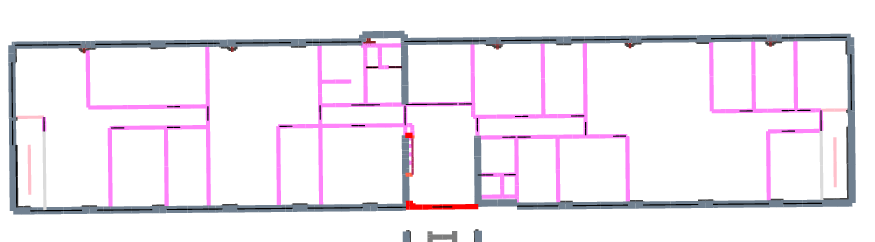
\includegraphics[width=7cm]{Gs2.png}
\caption{La légende est \emph{sous} la figure}
\end{centering}
\end{figure}
%



\begin{table}[htb]
\centering{}
\begin{tabular}{|l|l|}
\hline 
LAPIN & CHAT \\
\hline
CHEVAL  & ENCLUME \\
\hline
\end{tabular}
\caption{Cette légende  est \emph{sous} la table}
\label{tab:animaux}
\end{table}
 
\section{Quelques jolis exemples}

Les équations peuvent aussi être écrites en ligne en utilisant une seule fois le symbole \$ comme $E>100$ $$E>100$$

\begin{equation}
E >100
\label{eq:1}
\end{equation}

On peut observer dans \ref{eq:1}}
\begin{equation*}
E >100
\end{equation*}

\subsection{Poker face}

club, diamond, heart spade
$$\clubsuit, \diamondsuit, \heartsuit ,\spadesuit$$
\section{Chimie}

Les illustrations ci-dessous proviennent du package {\tt  chemfig}
\chemfig{A-B*5(-C-D*5(-X-Y-Z?)-E?-F-)} 

\definesubmol{&}{-[,,,,draw=none]}
\definesubmol{&&}{-[,,,2,draw=none]}
\chemfig{*6((-HO)-=*6(!&!{&&}HN(-CH_3)-[,,2]-(<OH)-)-=-(-HO)=)}
\subsection{Pile ou Face ? }

La probabilité d'obtenir k fois pile quand on lance $n$ fois la pièce

\begin{equation}
    P(k pile)   = {n \choose k} p^k (1-p)^{ n-k}
\end{equation}

Voici un exemple qui utilise une commande prédéfinie dans le fichier {\tt .tex}
\begin{equation}
\sm{k} \frac{1}{k^2}
\end{equation}
\subsection{Les pépites du copain d'Hardy}

\begin{equation}
  \frac{1}{\Bigl(\sqrt{\phi \sqrt{5}}-\phi\Bigr) e^{\frac25 \pi}} =
    1 + \frac{e^{-2\pi}} 
             {1+\frac{e^{-4\pi}} 
             {1+\frac{e^{-6\pi}}
             {1+\frac{e^{-8\pi}} 
             {1+\ldots} } } }
\end{equation}
\subsection{Utilisation d'alias}

La syntaxe : 
\begin{verbatim} 
    \newcommand{alias}{code Latex}
\end{verbatim}
permet de saisir plus rapidement des expressions complexes. 
Voir le début du source de ce document. Latex est utile non seulement pour
écrire des mathématiques, mais aussi pour en fabriquer.

\bear
\smu{n} \frac{1}{n^2} =  \frac{\pi^2}{6}
\ear

\bear
\zeta(s)= \smu{n} \frac{1}{n^s}
\ear

\subsection{What else do you expect ? }

Les équations de qui déjà ?

\begin{equation}
\begin{aligned}
    \nabla \times \vec{\mathbf{B}} -\, \frac1c\,
    \frac{\partial\vec{\mathbf{E}}}{\partial t} & = \frac{4\pi}{c}\vec{\mathbf{j}} \\  
    \nabla \cdot \vec{\mathbf{E}} & = 4 \pi \rho \\
    \nabla \times \vec{\mathbf{E}}\, +\, \frac1c\,
    \frac{\partial\vec{\mathbf{B}}}{\partial t} & = \vec{\mathbf{0}} \\
    \nabla \cdot \vec{\mathbf{B}} & = 0
\end{aligned}
\end{equation}
\section{Utilisation de l'alias \\sm}
$$\sm{k}$$
$$\smr{j}{1}{+\infty}$$
\section{Le monstre}
En mathématiques, le Monstre $M$ ou groupe de Fischer-Griess $F_1$ est le plus gros des 26 groupes simples sporadiques. Son ordre est
% L'étoile permet d'éviter la numérotation
\begin{eqnarray*}
246.320.59.76.112.133.17.19.23.29.31.41.47.59.71 \\
= 808 017 424 794 512 875 886 459 904 961 710 757 005 754 368 000 000 000 \\
\approx 8.10^{53}
\end{eqnarray*}

Pour en savoir plus googler "monstrous moonshine"
\begin{sudoku}
|2|5| | |3| |9| |1|.
| |1| | | |4| | | |.
|4| |7| | | |2| |8|.
| | |5|2| | | | | |.
| | | | |9|8|1| | |.
| |4| | | |3| | | |.
| | | |3|6| | |7|2|.
| |7| | | | | | |3|.
|9| |3| | | |6| |4|.
\end{sudoku}
\section{Satoshi in the glue ...}
"Le principe de ce système de paiement est de tenir à jour sur un très grand nombre de nœuds du réseau, un registre à la fois public et infalsifiable de toutes les transactions dont le montant est exprimé dans l'unité de compte bitcoin. Chaque bitcoin est identifiable depuis sa création, par un historique de toutes les transactions dans lesquelles il est impliqué. Les transactions sont reconnues valables par les signatures cryptographiques correspondantes qui ainsi les avalisent. Les bitcoins figurant dans les transactions dont un compte est bénéficiaire, peuvent être réutilisés par le titulaire de ce compte dans des transactions dont il sera l'émetteur. Il devra alors justifier au réseau que ce compte lui appartient au moyen d'une signature cryptographique créée à partir de sa clé privée. Les bitcoins ainsi échangés constituent une monnaie cryptographique, qui a vocation à être utilisée en tant que moyen de paiement.
Conçu en 2009 par un développeur non identifié utilisant le pseudonyme de Satoshi Nakamoto, le protocole a été employé pour la première fois dans un logiciel écrit par Nakamoto en C++ et publié sous licence libre MIT."\footnote{Source WikiPedia}
\section{Conclusion}
Il faut toujours écrire une conclusion. 
\begin{itemize}
  \item {\textbf GERONTE} - Latex c'est bien 
  \item {\textbf ALCESTE} - Je fais la même chose avec BureauOuvert.org
  \item {\textbf GERONTE} - En effet \dots
  \item[$\clubsuit$] En effet \dots
\end{itemize}
% 
%\begin{comment}
%\bibliographystyle{IEEEbib} %numérique
\bibliographystyle{utphys}
%\bibliographystyle{alpha}  %alphanumérique
\bibliography{ref}  % renvoie au fichier ref.bib dans lequel sont listé les références bibliographiques

%\end{comment}
{}
% \begin{IEEEbiography}
% [{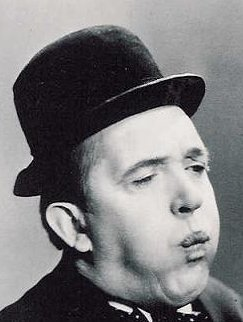
\includegraphics[width=2cm]{SLaurel.jpg}}]
% {Stan Laurel } era un actor cómico, escritor y director británico,
% famoso por ser miembro del famoso dúo cómico junto a Oliver Hardy 

% \end{IEEEbiography}

% \begin{IEEEbiography}
% [{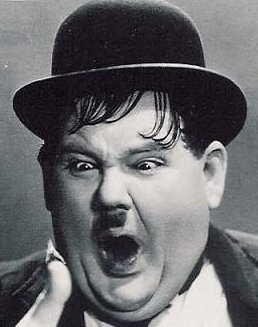
\includegraphics[width=2cm]{OHardy.jpg}}]
% {Oliver Hardy} Homonyme du mentor de Srinivasa Ramanujan
% \end{IEEEbiography}

\end{document}
